
\section{Trailer}\label{sec:trailer}

\renewcommand{\kapitelautor}{Autor: Markus Böheim}

Für den Trailer wird Adobe Premiere Pro verwendet. Das Hauptziel des Trailers
ist es das Gameplay actionreich zu präsentieren, damit es Interesse weckt und um die Grafiken hervorzuheben.
Die Zielgruppe von Forty-Five sind junge Menschen die bereits Interesse an dem Genre haben, also muss ein gewisser
Vergleich oder Ähnlichkeit im Trailer zu anderen Spielen in diesem Genre sein, damit der Spieler weiß, worum es geht.
Eine Grobe Idee für den Trailer oder Skript in Form eines Storyboards, sorgt bei der Umsetzung des Trailers für einen
schnelleren Workflow sowohl bei der Pre-Production als auch bei dem Zusammenschnitt.
Als Referenz wird der Trailer von \quoted{Slay the Spire} vorgenommen, um einen Anhaltspunkt für die Geschwindigkeit zu haben.
Zuerst werden mit dem Storyboard die notwendigen Szenen aufgenommen. Dafür wird eine Version des Spiels benötigt ohne Musik, da diese beim Schnitt Probleme bereitet. Nach der Aufnahme werden nach der Anleitung des geschriebenen Storyboards die aufgenommenen Clips zusammengeschnitten. Zooms helfen, um mehr Fokus auf eine bestimme Aktion oder ein Objekt zu bringen. Keyframes – auf Deutsch Schlüsselbilder – Keyframes legen Start- und Endpunkt einer Animation fest. Mit Keyframes ist es möglich, einen Zoom Effekt in Schnittprogrammen zu erstellen, indem man beispielsweise einen Startpunkt mit der Skalierung 100 und einen Endpunkt mit der Skalierung 110 setzt. Das ist allerdings nur eine lineare Kurve, die unnatürlich aussieht. Mit Ease-In und Ease-Out Funktionen wird das Skalieren dadurch natürlicher, welche per Rechtsklick auf den Keyframe eingestellt werden können.

\begin{figure}[H]
    \centering
    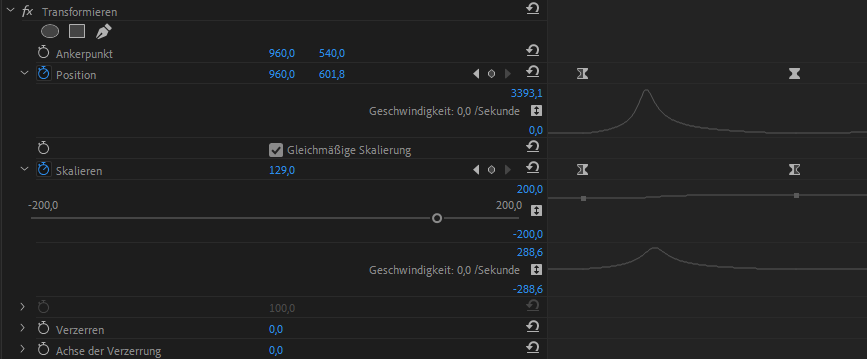
\includegraphics[width=0.6\textwidth]{easeInOut.png}
    \caption{Ease-In/Out Zoom im Trailer}
\end{figure}

Die Musik im Trailer ist lizenzfrei unter dem Link \url{https://www.youtube.com/watch?v=KIhO3u0xuhQ} zu finden und wird gewählt, da die Instrumente und Soundgeräusche zum wilden Westen passen und eine dramatische, ernste Stimmung hat. Da der Trailer nur grob eine Minute lang ist und das Musikstück grob drei Minuten lang ist, muss der Song auf den Trailer angepasst werden.
Premiere Pro bietet eine \quoted{Remix} Funktion, welche unter dem \quoted{Essential Sound}
Reiter zu finden ist, die es einem erlaubt, die Länge eines Songs anzupassen, ohne dass der Rhythmus des Songs dabei unterbrochen wird.

\begin{figure}[H]
    \centering
    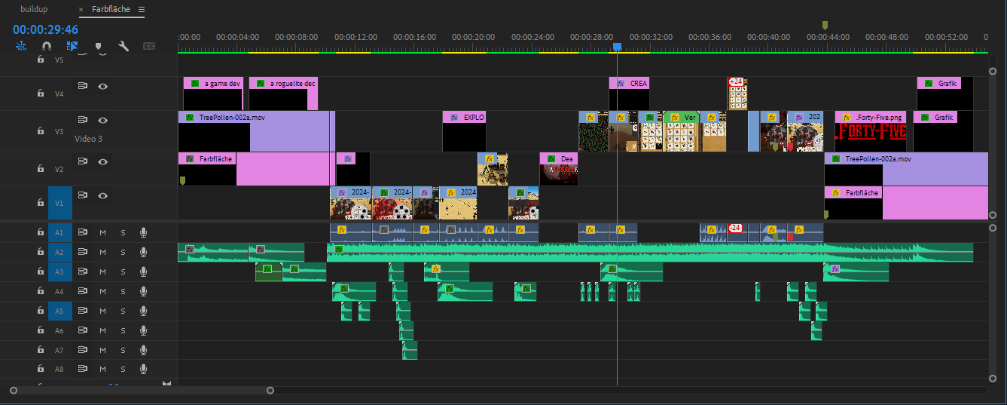
\includegraphics[width=0.6\textwidth]{schnittfenster.png}
    \caption{Arbeitsfläche des Trailers}
\end{figure}

Das Audio beziehungsweise die Vertonung ist genauso wichtig, wie das Video an sich selbst.
Für Texte, die erscheinen, wird ein Soundeffekt verwendet, welcher einem wischen ähnelt.
Die Sounds für den Trailer werden von Pixabay’s kosten- und lizenzfreier Audiobibliothek genommen und werden von der
Lautstärke so angepasst, dass diese mit den anderen Audiospuren inklusive des Musikstücks den Richtwert -6dB nicht
überschreiten. Dieser Audiopegel von -6dB sorgt dafür, dass das Audio ausreichend \quoted{Headroom} beziehungsweise Spielraum
hat, um plötzliche Laute Geräusche abzufangen, ohne dass diese übersteuern. Abschließend wird der Trailer in 1080p und 60 Bildern pro Sekunde exportiert, mit einer Bitrate von 36Mbit/s, um das Video konform für die Veröffentlichung in sozialen Medien zu machen. Die Bitrate sagt aus, wie viele Daten pro Sekunde übertragen werden, was die Qualität und Dateigröße beeinflusst.



% resets author
\renewcommand{\kapitelautor}{}
